\chapter{Inventur}
\label{Inventur}
F�r die Inventur der Betriebsmittel steht ein eigenes Tool zur Verf�gung.
Sie finden es unter dem Men�punkt Inventar->Inventur.
Hier k�nnen sie Ausw�hlen f�r welchen Raum und/oder welche Person sie die Inventur durchf�hren.
Klicken Sie auf 'Inventur starten' um zu beginnen.
\begin{figure}
	\centering
	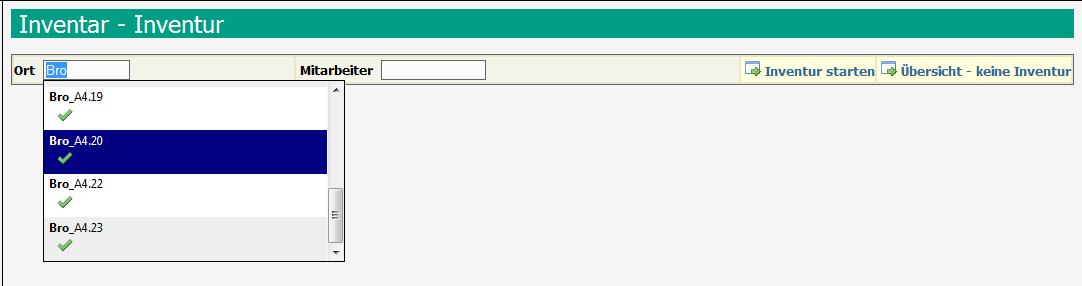
\includegraphics[width=0.80\textwidth]{Inventar_inventur_autocomplete.png}
	\caption{Raumauswahl}
	\label{Raumauswahl}
\end{figure}

Sie k�nnen nun die vorhandenen Betriebsmittel mit dem Barcodescanner nacheinander erfassen.
Bei diesen Betriebsmittel wird nun automatisch das Inventurdatum gesetzt, der Name der Person welche die Inventur durchgef�hrt hat und das Betriebsmittel wird automatisch dem ausgew�hlten Raum und/oder der Person zugeordnet.
\begin{figure}
	\centering
	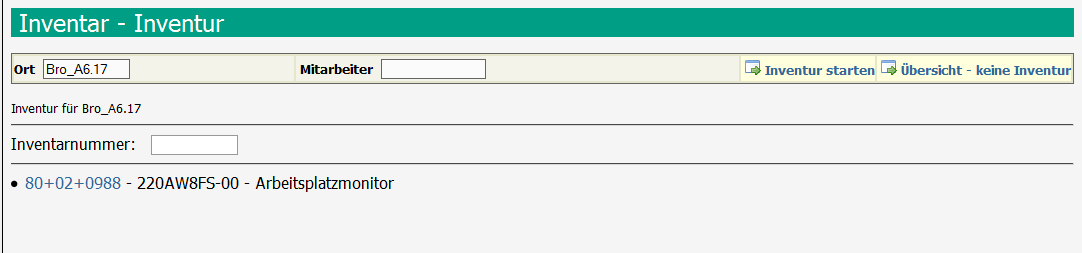
\includegraphics[width=0.80\textwidth]{Inventar_inventur.png}
	\caption{Inventur der Betriebsmittel}
	\label{Inventur der Betriebsmittel}
\end{figure}
\\
Nachdem Sie alle Ger�te in diesem Raum oder von dieser Person erfasst haben, k�nnen Sie sich eine Liste der Ger�te anzeigen lassen, die sich in diesem Raum oder im Besitz der Person befinden sollten, aber in den letzten 20 Wochen nicht erfasst wurden.
Klicken Sie dazu auf den Punkt '�bersicht - keine Inventur'.\\
Sie k�nnen hier die nicht erfassten Ger�te auscheiden oder in einen Dummy-Raum zur weiteren Bearbeitung verschieben.\\
\begin{figure}
	\centering
	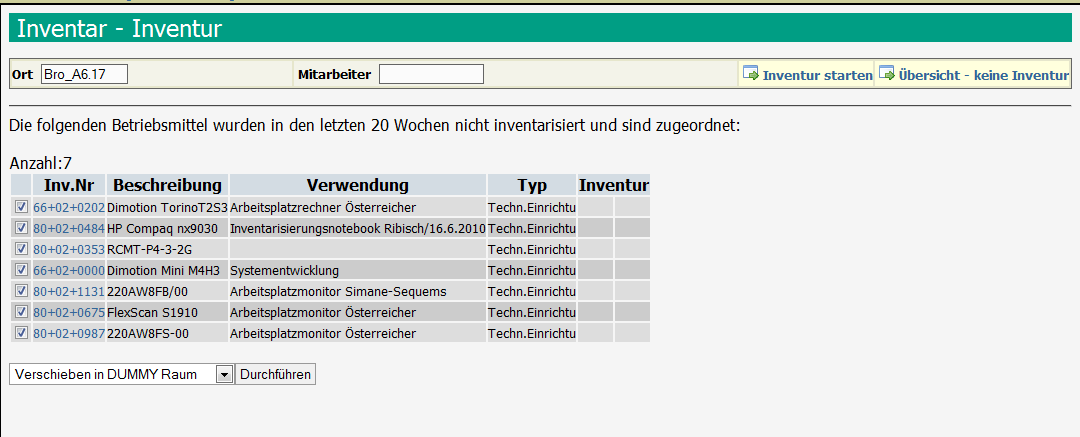
\includegraphics[width=0.80\textwidth]{Inventar_inventur_keine_inventur.png}
	\caption{�bersucht der Betriebsmittel die nicht erfasst wurden}
	\label{�bersicht der Betriebsmittel die nicht erfasst wurden}
\end{figure}